\subsection{Mission Specific Auxiliary Tools}

\subsubsection{Stabilizing Cap Positioning Extension}

One of the specialized systems developed for Kamikaze is the Stabilizing Cap Positioning Extension (SCPE). While Kamikaze installs a new thermistor, the SCPE (Figure \ref{fig:scpe}) secures the thermistor cap in place, ensuring perfect alignment.

\hspace{10pt} The mechanism's smooth and controlled extension is provided by a telescopic ball-bearing slide, which is like those found in drawer runners. A 2.5-inch diameter cup at the top provides a little amount of alignment tolerance, guaranteeing a firm but flexible hold on the cap.

\hspace{10pt} The extension lengthens as the SCPE holds onto the cap and Kamikaze lowers, keeping the cap in place. The extension shrinks as Kamikaze rises with the thermistor, holding the cap firmly in place and facilitating a smooth hookup.

\subsubsection{Liquid Sample Acquiring System}

To enable efficient and flexible liquid sample collection, a modular design approach (Figure \ref{fig:pump}) was implemented. This design allows for straightforward assembly, disassembly, and maintenance of individual components, thereby improving both convenience and system reliability during the sampling process. To further ensure optimal functionality under high-pressure conditions, the system incorporates a mini pump with a flow rate of 80 L/h, which was tested underwater to validate its performance. Additionally, a collection bottle featuring a user-friendly disassembly mechanism was integrated, easing the sample retrieval process and confirming its compatibility within the overall system.

\subsubsection{Jelly Collecting Shutter Mechanism}

A specialized mechanism has been developed to collect and transport a jelly-like object filled with water to the surface. The system consists of a sealed acrylic tube, closed at the top, with a pneumatically controlled shutter at the bottom. When the pilot successfully guides the jelly inside the tube, the shutter activates, preventing it from drifting away while allowing water to flow freely. This design (Figure \ref{fig:jelly}) ensures that the jelly remains contained within the tube as it ascends due to buoyancy, enabling controlled and efficient transport to the surface.

\subsubsection{Customized Hook}

A customized hook mechanism has been developed to efficiently collect chenille strips (pipe cleaners) from the water surface. Since the strips float on the surface, they cannot be gripped using the ROV’s main gripper. Positioned at the top of the ROV, the hook (Figure \ref{fig:hook}) is strategically designed to maximize the number of strips gathered in a single attempt. To further enhance the mechanism’s effectiveness, Velcro can be added to ensure the strips stick within the hook securely. This design improves the ROV’s efficiency in completing the task, ensuring a higher collection rate.

\begin{figure}[ht!] 
    \centering
    \begin{subfigure}[b]{0.49\columnwidth} 
        \centering
        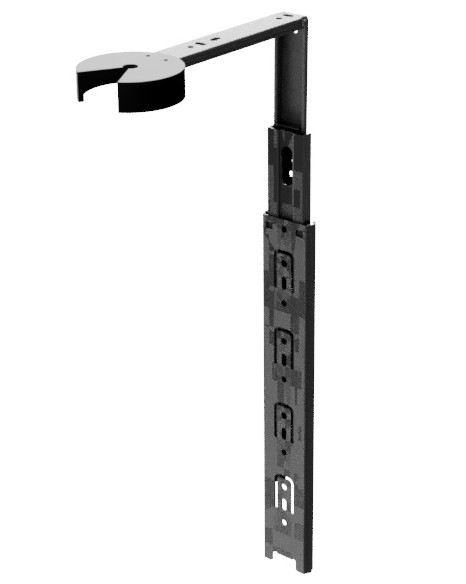
\includegraphics[height=3cm]{Sections/2Design Rationale/images/Stabilizing Cap Positioning Extension (SCPE) .jpg}
        \caption{\scriptsize Stabilizing Cap Positioning Extension.}
        \label{fig:scpe}
    \end{subfigure}
    \hfill
    \begin{subfigure}[b]{0.49\columnwidth}
        \centering
        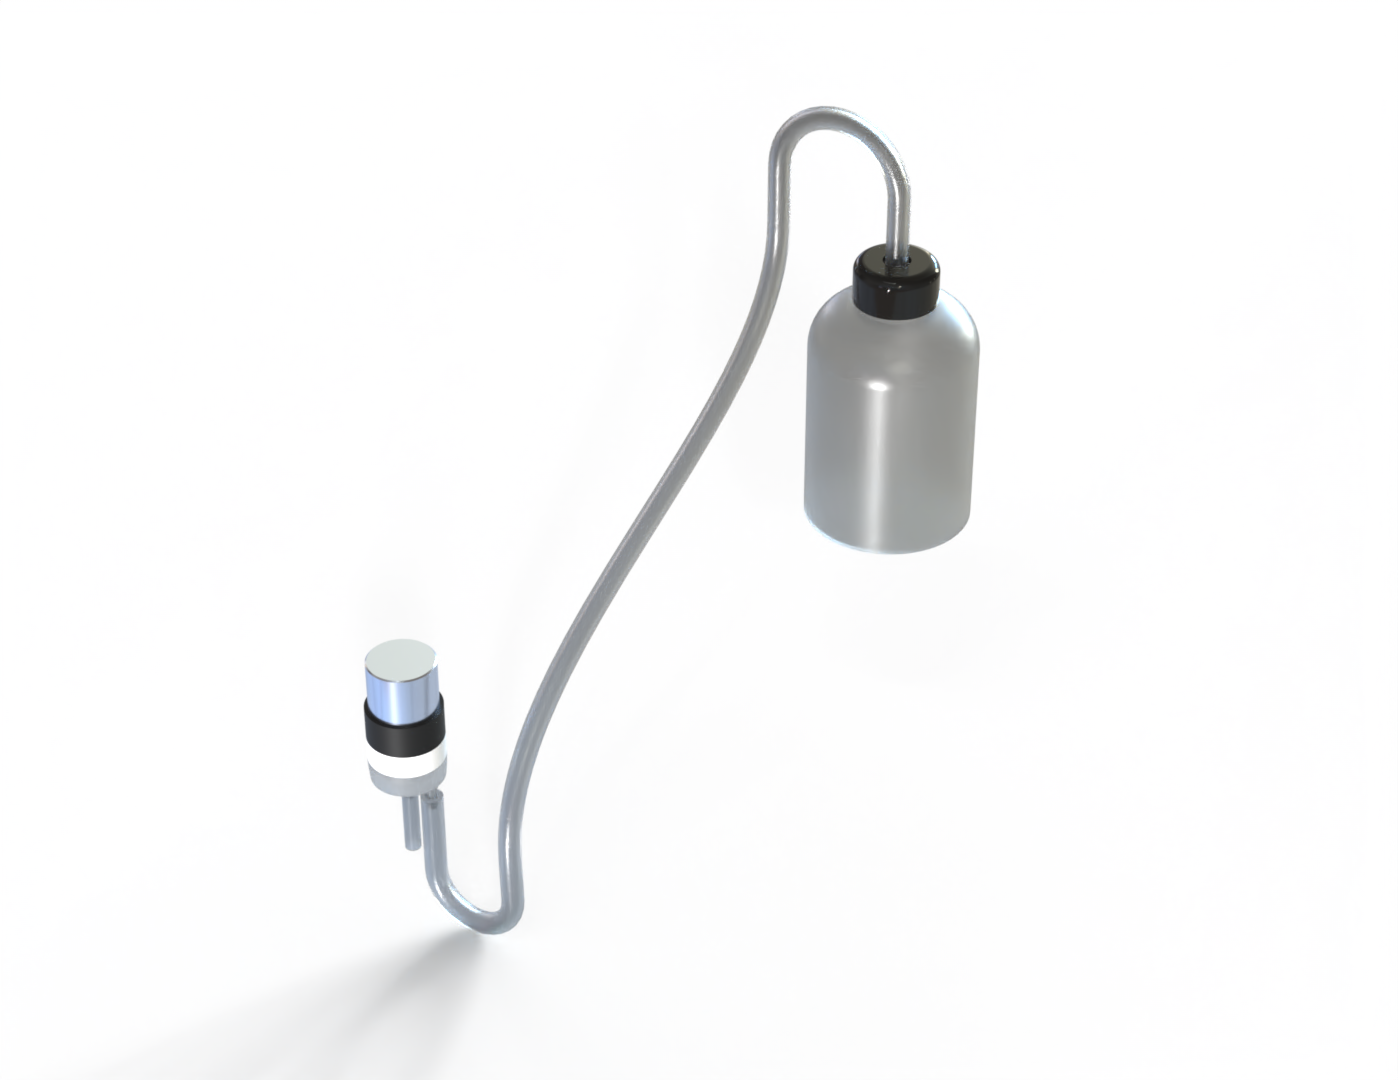
\includegraphics[width=\linewidth]{Sections/2Design Rationale/images/Pump.png}
        \caption{\scriptsize Liquid Sample Acquiring System.}
        \label{fig:pump}
    \end{subfigure}

    \vspace{0.2cm}

    \begin{subfigure}[b]{0.49\columnwidth}
        \centering
        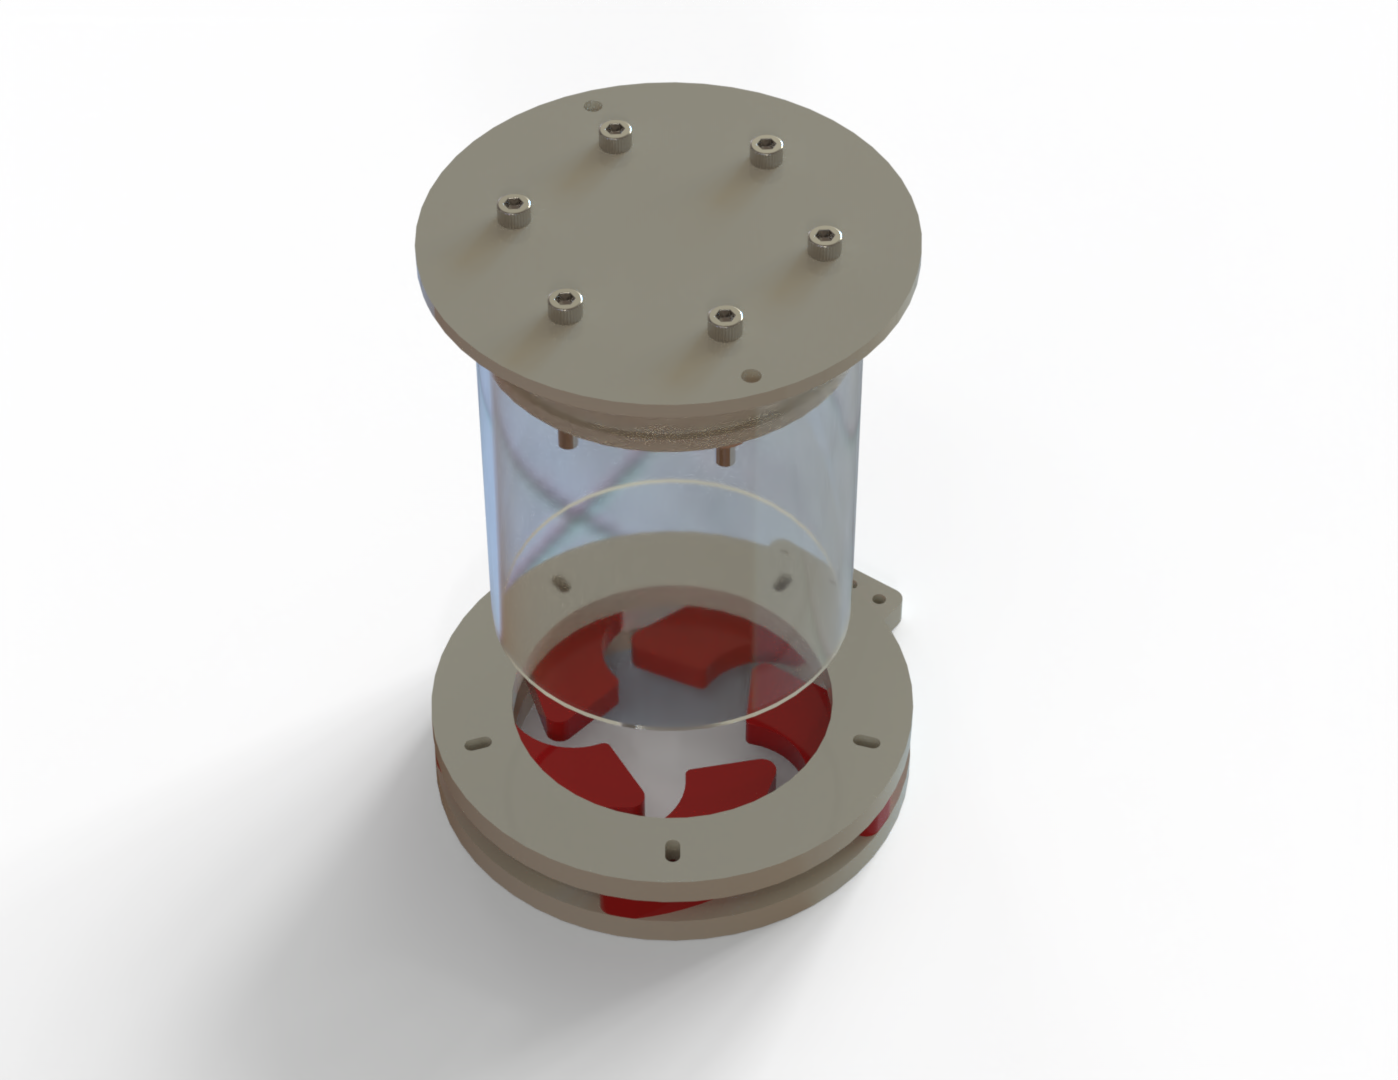
\includegraphics[width=\linewidth]{Sections/2Design Rationale/images/Jelly.png}
        \caption{\scriptsize Jelly Collecting Shutter Mechanism.}
        \label{fig:jelly}
    \end{subfigure}
    \hfill
    \begin{subfigure}[b]{0.49\columnwidth}
        \centering
        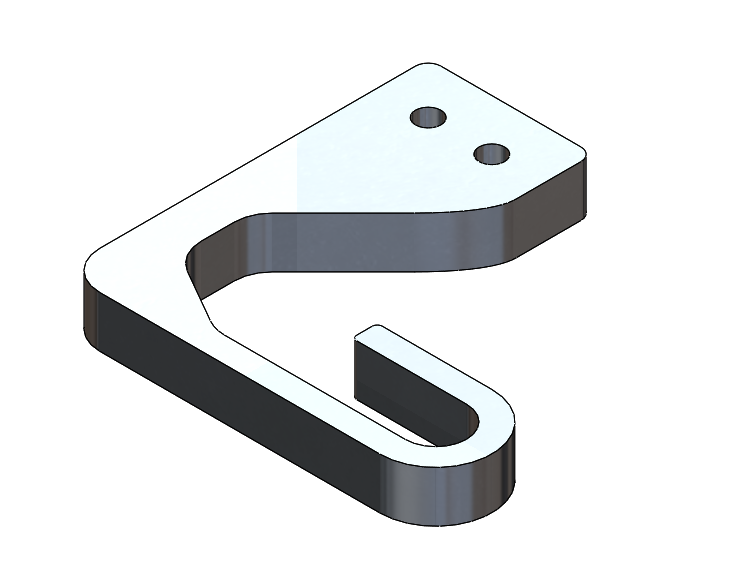
\includegraphics[width=\linewidth]{Sections/2Design Rationale/images/Hook.png} 
        \caption{\scriptsize Customized Hook.}
        \label{fig:hook}
    \end{subfigure}

    \caption{Kamikaze's Mission-Specific Tools.}
    \label{fig:mission_specific_tools}

\end{figure}

\subsubsection{Vertical Profiling Float}

EJUST Robotics Clun supports the National Science Foundation (NSF)-funded GO-BGC project’s mission to build a global network of chemical and biological sensors for ocean health monitoring. As part of this initiative, our team has developed Fat Man, a vertical profiling float designed for ocean observation and data collection. This float enhances the ability to monitor key environmental parameters, providing valuable insights into ocean dynamics and contributing to global research efforts on climate change.

\begin{figure}[h]
    \centering
    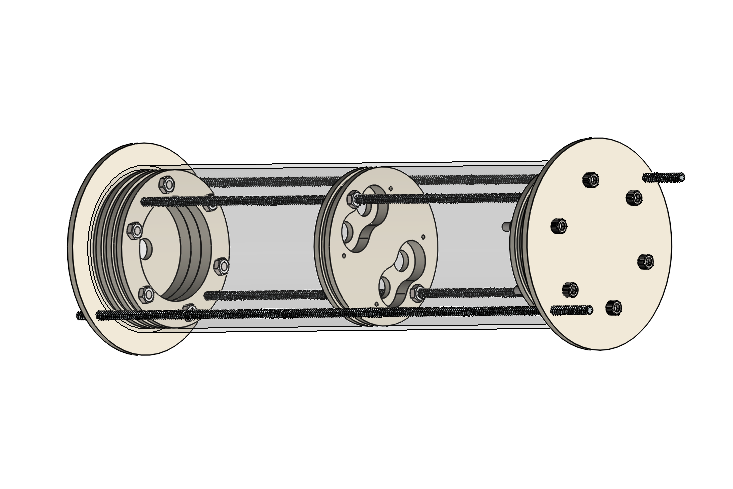
\includegraphics[height=9cm]{Sections/2Design Rationale/images/float.png}
    \caption{E-JUST Vertical Profiling Float, Fat Man.}
    \label{fig:Float}
\end{figure}

Fat Man is constructed from transparent acrylic, allowing visual inspection and error detection, and is divided into two sections by an HDPE disk to separate the electrical components from the water chamber. A suction system with peristaltic pumps enables precise buoyancy control by regulating water intake and release. The electrical system, powered by an STM32 microcontroller, integrates a depth sensor, motor driver, and NRF24L01 radio module for real-time data collection and transmission. Supported by NiMH batteries, the system ensures stable operation, reinforcing EJUST Robotics Club's commitment to advancing ocean research and technology.